\documentclass[12pt, a4paper]{article}

\usepackage[utf8]{inputenc}
% Limit the page margin to only 1 inch.
\usepackage[margin=1in]{geometry}

%Imports biblatex package
\usepackage[
backend=biber,
style=alphabetic
]{biblatex}
\addbibresource{../../algs4e.bib}

% Enables the `align' environment.
\usepackage{amsmath}
% Provides useful environments, such as:
% - \begin{proof} ...\end{proof}
\usepackage{amsthm}
\usepackage[most]{tcolorbox}

\newtheorem*{proposition}{Proposition}

% Enables using \mathbb{}, for example \mathbb{N} for the set of natural numbers.
\usepackage{amssymb}

% Allows using letters in enumerate list environment. Use, for example:
%\begin{enumerate}[label=(\alph*)]
% ...
%\end{enumerate}
\usepackage[inline]{enumitem}

% Enable importing external graphic files and provides useful commannds, like \graphicspath{}
\usepackage{graphicx}
% Images are located in a directory called images in the current directory.
\graphicspath{{./images/}}

% Make links look better by default.
% See: https://tex.stackexchange.com/questions/823/remove-ugly-borders-around-clickable-cross-references-and-hyperlinks
\usepackage[hidelinks]{hyperref}
\usepackage{xcolor}
\hypersetup{
	colorlinks,
	linkcolor={red!50!black},
	citecolor={blue!50!black},
	urlcolor={blue!80!black}
}


% Code Listings. Source:
% https://stackoverflow.com/questions/3175105/inserting-code-in-this-latex-document-with-indentation
\usepackage{listings}
\usepackage{color}

\definecolor{dkgreen}{rgb}{0,0.6,0}
\definecolor{gray}{rgb}{0.5,0.5,0.5}
\definecolor{mauve}{rgb}{0.58,0,0.82}

\lstset{frame=tb,
	language=Java,
	aboveskip=3mm,
	belowskip=3mm,
	showstringspaces=false,
	columns=flexible,
	basicstyle={\small\ttfamily},
	numbers=none,
	numberstyle=\tiny\color{gray},
	keywordstyle=\color{blue},
	commentstyle=\color{dkgreen},
	stringstyle=\color{mauve},
	breaklines=true,
	breakatwhitespace=true,
	tabsize=3
}

\newcommand{\prob}{\text{P}}
%\newcommand{\complement}{\mathsf{c}}

% Define an environment called "ex" (for Exercise) so that I can do: \begin{ex}{1.5}...\end{ex}
\newenvironment{ex}[2][Exercise]
{\par\medskip\noindent \textbf{#1 #2.}}
{\medskip}

% Define a solution environment, similar to ex (exercise) environment.
\newenvironment{sol}[1][Solution]
{\par\medskip\noindent \textbf{#1.} }
{\medskip}

\begin{document}
	\noindent Sergio E. Garcia Tapia \hfill
	
	\noindent \emph{Algorithms} by Sedgewick and Wayne (4th edition) \cite{sedgewick_wayne}\hfill
	
	\noindent December 1st, 2024\hfill 
	\section*{3.2: Binary Search Trees}
	\begin{ex}{1}
		Draw the BST that results when you insert the keys \texttt{E A S Y Q U E S T I O N},
		in that order (associating the value \texttt{i} with the \texttt{i}th key, as per the
		convention in the text) into an initially empty tree. How many compares are needed
		to build the tree?
	\end{ex}
	\begin{sol}
		The sequence of binary search trees is shown in Figure~\ref{fig:ex-01}. The boxes next
		two the root show the number of compares necessary to complete the insertion at
		that step. The sequence of compare counts is: 0, 1, 1, 2, 2, 3, 1, 2, 4, 3, 4, 5.
		Adding gives a total of 28 compares.
		\begin{figure}
			\centering
			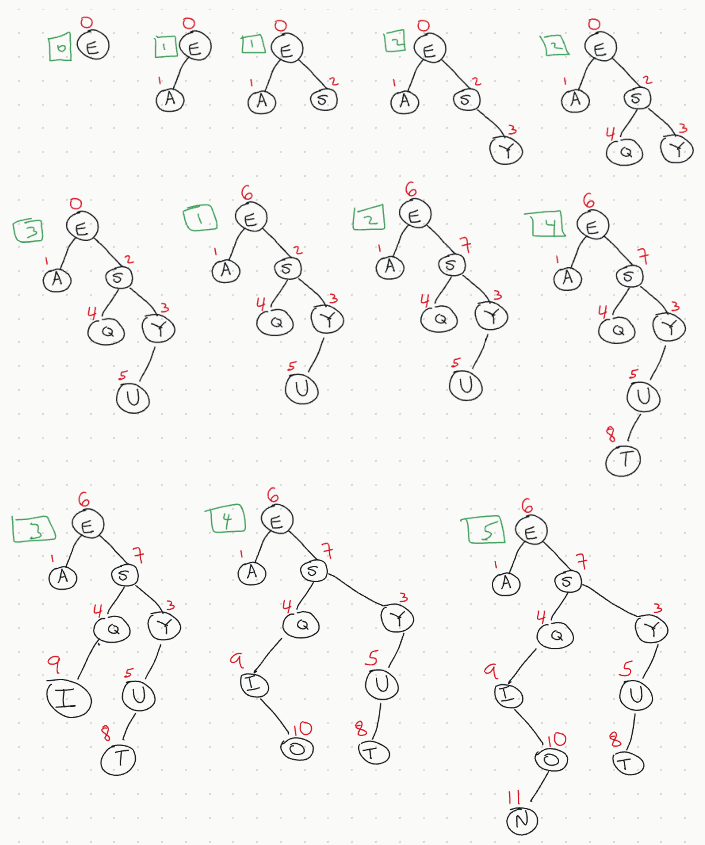
\includegraphics[width=0.7\textwidth]{exercise-01}
			\caption{Exercise 1: Sequence of trees formed when inserting the keys \texttt{E A S Y Q U E S T I O N}
			into a binary search tree.}
			\label{fig:ex-01}
		\end{figure}
	\end{sol}
	\begin{ex}{2}
		Inserting the keys in the order \texttt{A X C S E R H} into an initially empty BST
		gives a worst-case tree where every node has one null link, except one at the bottom,
		which has two null links. Give five other orderings of these keys that produce
		worst-case trees. 
	\end{ex}
	\begin{sol}
		We can insert them in the following ways:
		\begin{enumerate}[label=(\roman*)]
			\item \texttt{A X C S E R H} (given).
			\item \texttt{X S R H E C A}.
			\item \texttt{A C E H R S X}.
			\item \texttt{X A S C R E H}.
			\item \texttt{X A S R H E C}.
			\item \texttt{A X C E H R S}.
		\end{enumerate}
		See Figure~\ref{fig:ex-02}.
		\begin{figure}
			\centering
			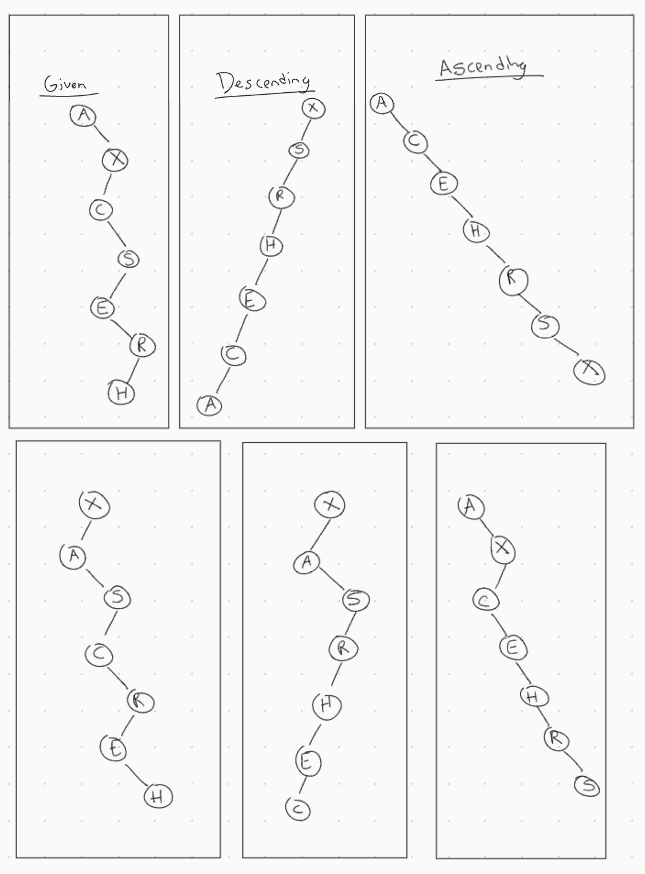
\includegraphics[width=0.7\textwidth]{exercise-02}
			\caption{Exercise 2: Worst-case binary search trees created by inserting the
			keys \texttt{A X C S E R H} into an initially empty tree in a particular order}
			\label{fig:ex-02}
		\end{figure}
	\end{sol}
	\begin{ex}{3}
		Give five orderings of the keys \texttt{A X C S E R H} that, when inserted into an
		initially empty BST, produce the \emph{best-case} tree.
	\end{ex}
	\begin{sol}
		\begin{enumerate}[label=(\roman*)]
			\item \texttt{H C S A E R X}.
			\item \texttt{H S C A E R X}.
			\item \texttt{H S C E A X R}.
			\item \texttt{H S R X C A E}.
			\item \texttt{H S X R C A E}.
		\end{enumerate}
		These all result in the same tree, depicted in Figure~\ref{fig:ex-03}.
		\begin{figure}
			\centering
			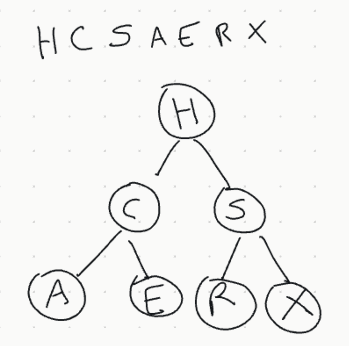
\includegraphics[width=0.3\textwidth]{exercise-03}
			\caption{Exercise 3: Best-case binary search trees created by inserting the
				keys \texttt{A X C S E R H} into an initially empty tree in a particular order}
			\label{fig:ex-03}
		\end{figure}
	\end{sol}
	\begin{ex}{4}
		Suppose that a certain BST has keys that are integers between \texttt{1} and \texttt{10},
		and we search for \texttt{5}. Which sequence below \emph{cannot} be the sequence
		of keys examined?
		\begin{enumerate}[label=(\alph*)]
			\item \texttt{10, 9, 8, 7, 6, 5}
			\item \texttt{4, 10, 8, 6, 5}
			\item \texttt{1, 10, 2, 9, 3, 8, 4, 7, 6, 5}
			\item \texttt{2, 7, 3, 8, 4, 5}
			\item \texttt{1, 2, 10, 4, 8, 5}
		\end{enumerate}
	\end{ex}
	\begin{sol}
		\begin{enumerate}[label=(\alph*)]
			\item This is a valid sequence. For example, this could be a tree where the
			keys were inserted in descending order.
			\item This is a valid sequence.
			\item This is a valid sequence.
			\item This sequence cannot happen. The sequence of compares suggests the following:
			\begin{enumerate}[label=(\roman*)]
				\item 2 is the root, and 5 is larger, so we go right.
				\item 5 is smaller than 7, so we go left.
				\item 5 is smaller than 3, so we go right.
				\item 5 is compared against 8.
			\end{enumerate}
			This last step is impossible because since 8 is larger than 7, but it
			appears on the subtree rooted at its left child, consisting of smaller
			keys,  a contradiction.
			\item This is a valid sequence.
		\end{enumerate}
	\end{sol}
		\begin{ex}{5}
		Suppose that we have an estimate ahead of time of how often search keys are
		to be accessed in a BST, and the freedom to insert them in any order that we
		desire. Should the keys be inserted into the tree in increasing order, decreasing
		order of likely frequency of access, or some other order? Explain your answer.
	\end{ex}
	\begin{sol}
		Increasing order is not desirable because it leads to a worst-case tree where
		every internal node hade has 1 null link and the leaf node has 2 null links
		(in essence, a linked list).
		
		Decreasing order of likely frequency of access biases towards the most frequency
		accessed nodes. However, if that order corresponds to the increasing or decreasing
		order of the keys, for example, then we may again have a worst-case tree.
		
		The safest thing to do is to insert them in an order that yields a balanced tree.
		Suppose that there are $n$ keys, and suppose we place them in sorted order,
		$k_0,k_1,\ldots,k_{n-1}$, so that $k_{i-1} \leq k_{i}$ for all $1\leq i\leq n$.
		Let \texttt{lo = 0}, and \texttt{hi = n - 1}
		Then we can insert them as follows:
		\begin{enumerate}[label=(\roman*)]
			\item If \texttt{lo > hi}, stop.
			\item Compute the middle key at index \texttt{mid = lo + (hi - lo) / 2}.
			This key $k_{mid}$ is the root.
			\item Set the left child of $k_{mid}$ to the tree resulting from (recursively) applying
			the algorithm to the subset of keys $k_0,\ldots,k_{mid-1}$.
			\item Set the right child of $k_{mid}$ to the tree resulting from (recursively) applying
			the algorithm to the subset of keys $k_{mid+1},\ldots,k_{hi}$.
		\end{enumerate}
		Notice this is effectively placing the partitioning the array like quicksort.
	\end{sol}
	\begin{ex}{6}
		Add to \texttt{BST} a method \texttt{height()} that computes the height of the tree.
		Develop two implementations: a recursive method (which takes linear time and space
		proportional to the height), and a method like \texttt{size()} that adds a field to
		each node in the tree (and takes linear space and constant time per query).
	\end{ex}
	\begin{sol}
		See \texttt{com.segarciat.algs4.ch3.sec2.ex06.BST}.
	\end{sol}
	\begin{ex}{7}
		Add to \texttt{BST} a recursive method \texttt{avgCompares()} that computes the average
		number of compares reuired by a random search hit in a given BST (the internal path length
		of the tree divided by its size, plus one). Develop two implementations: a recursive method
		(which takes linear time and space proportional to the height), and a method like
		\texttt{size()} that adds a field to each node in the tree (and takes linear space and
		constant time per query).
	\end{ex}
	\begin{sol}
		See \texttt{com.segarciat.algs4.ch3.sec2.ex07.BST}.
	\end{sol}
	\begin{ex}{8}
		Write a static method \texttt{optCompares()} that takes an integer argument \texttt{n}
		and computes the number of compares required by a random search hit in an optional
		(perfectly balanced) BST with \texttt{n} nodes, where all the null links are on the
		same level if the number of links is a power of 2 or one of two levels otherwise.
	\end{ex}
	\begin{sol}
		See \texttt{com.segarciat.algs4.ch3.sec2.ex08.BSTOptCompares}.
	\end{sol}
	\begin{ex}{9}
		Draw all the different BST shapes that can result when \texttt{n} keys are inserted
		into an initially empty tree, for \texttt{n} = \texttt{2, 3, 4, 5}, and \texttt{6}.
	\end{ex}
	\begin{sol}
		See Figure~\ref{fig:ex-09} for \texttt{n = 2, 3, 4}. I considered the reflections
		on the $y$-axis to be of the same shape, so I chose not to draw them.
		\begin{figure}
			\centering
			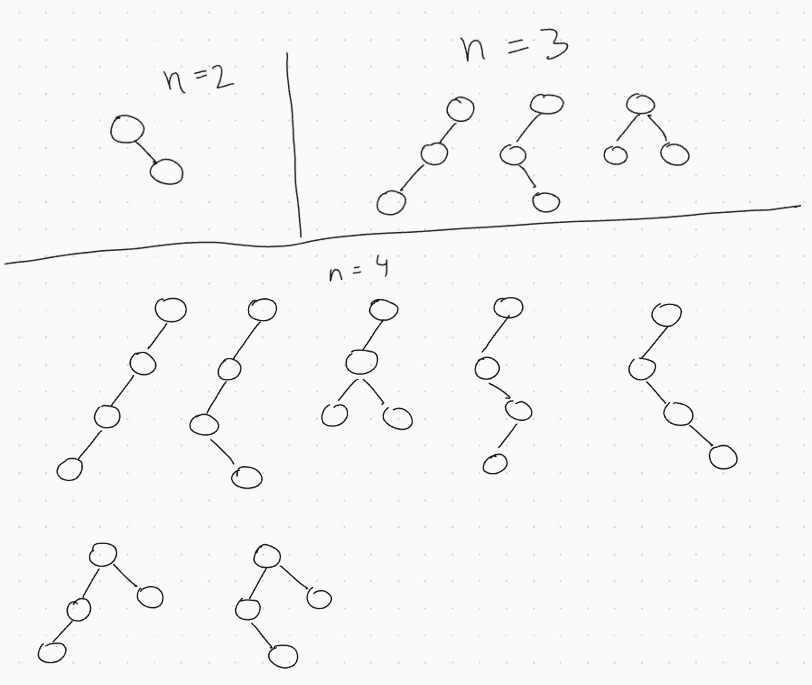
\includegraphics[width=0.6\textwidth]{exercise-09}
			\caption{Exercise 9: All binary-search tree shapes for $n=2,3,4$ vertices.}
			\label{fig:ex-09}
		\end{figure}
	\end{sol}
	\begin{ex}{10}
		Write a test client for \texttt{BST} that tests the implementations of \texttt{min()},
		\texttt{max()}, \texttt{floor()}, \texttt{ceiling()}, \texttt{select()}, \texttt{rank()},
		\texttt{delete()}, \texttt{deleteMin()}, \texttt{deleteMax()}, and \texttt{keys()} that
		are given in the text. Start with the standard indexing client given on page 370.
		Add code to take additional command-line arguments, as appropriate.
	\end{ex}
	\begin{ex}{11}
		How many binary tree shapes of $n$ nodes are there with height $n$? How many different
		ways are there to insert $n$ different keys into an initially empty BST that result
		in a tree of height $n-1$? (See \textbf{Exercise 3.2.2})
	\end{ex}
	\begin{sol}
		There are 0 binary tree shapes of $n$ nodes with height $n$, because the height
		of a tree is the maximum depth among all of the nodes, and the smallest node
		is that of the root which is $0$.
		
		However, there are $2^{n-1}$ binary ways to insert $n$ different keys into an
		initially empty BST that results in a tree of height $n-1$. A path from the root
		to the leaf in such a tree of height $n-1$ consists of a sequence of left and right
		turns. At each node, we make a decision of whether to go left or right. Since there
		are $n-1$ edges, and we choose to lean left or right at each step, we get $2^{n-1}$.
	\end{sol}
	\begin{ex}{12}
		Develop a \texttt{BST} implementation that omits \texttt{rank()} and \texttt{select()}
		and does not use a count field in \texttt{Node}.
	\end{ex}
	\begin{sol}
		See \texttt{com.segarciat.algs4.ch3.sec2.ex11.BST}.
	\end{sol}
	\begin{ex}{13}
		Give nonrecursive implementations of \texttt{get()} and \texttt{put()} for \texttt{BST}.
		The implementation of \texttt{put()} is more complicated because of the need to save
		a pointer to the parent node to link in the new node at the bottom. Also, you need
		a separate pass to check whether the key is already in the table because of the need
		to update the counts. Since there are many more searches than inserts in performance-critical
		implementations, using this code for \texttt{get()} is justified; the corresponding change
		for \texttt{put()} might not be noticed.
	\end{ex}
	\begin{sol}
		See \texttt{com.segarciat.algs4.ch3.sec2.ex13.BSTNonRec}.
	\end{sol}
	\begin{ex}{14}
		Give nonrecursive implementations of \texttt{min()}, \texttt{max()}, \texttt{floor()},
		\texttt{ceiling()}, \texttt{rank()}, \texttt{select()}, and \texttt{keys()}.
	\end{ex}
	\begin{sol}
		See \texttt{com.segarciat.algs4.ch3.sec2.ex14.BSTNonRec}.
	\end{sol}
	\begin{ex}{15}
		Give the sequences of nodes examined when the methods in \texttt{BST} are used to
		compute each of the following quantities for the tree drawn in Figure~\ref{fig:ex-15}.
		\begin{figure}
			\centering
			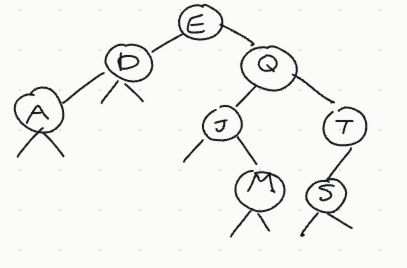
\includegraphics[width=0.4\textwidth]{exercise-15}
			\caption{Exercise 15: Binary Search Tree}
			\label{fig:ex-15}
		\end{figure}
		\begin{enumerate}[label=(\alph*)]
			\item \texttt{floor("Q")}
			\item \texttt{select(5)}
			\item \texttt{ceiling("Q")}
			\item \texttt{rank("J")}
			\item \texttt{size("D", "T")}
			\item \texttt{keys("D", "T")}
		\end{enumerate}
	\end{ex}
	\begin{sol}
		\begin{enumerate}[label=(\alph*)]
			\item \texttt{"E"}, \texttt{"Q"}
			\item \texttt{"E"}, \texttt{"Q"}
			\item \texttt{"E"}, \texttt{"Q"}
			\item \texttt{"E"}, \texttt{"Q"}, \texttt{"J"}
			\item First the \texttt{contains(hi)} call leads to the following
			sequence: \texttt{"E"}, \texttt{"Q"}, \texttt{"T"}. Then the call
			to \texttt{rank(hi)} leads to the sequence \texttt{"E"}, \texttt{"Q"},
			\texttt{"T"}. Then, the call \texttt{rank(lo)} leads to the sequence
			\texttt{"E", "D"}.
			\item \texttt{"E"}, \texttt{"D"}, \texttt{"Q"}, \texttt{"J"}, \texttt{"M"},
			\texttt{"T"}
		\end{enumerate}
	\end{sol}
	\pagebreak
	\printbibliography
\end{document}